\documentclass[../piano-di-qualifica.tex]{subfiles}

\begin{document}
In questa sezione vengono resi noti i risultati dei test relativi al periodo di revisione dei documenti e requisiti, mediante l'utilizzo delle metriche descritte nelle sezioni precedenti.
I risultati possono coincidere o meno con i valori desiderati dal gruppo, nel caso non coincidessero verrà fatta un ulteriore analisi per il miglioramento visibile nella sezione appendice B.

\subsection{Primo periodo (RR)}
\label{sub:primo_periodo}
Durante questo periodo è stata sottoposta ad una precisa attività di verifica tutta la documentazione da presentare in ingresso in sede di Revisione dei Requisiti.
I verificatori inizialmente hanno effettuato l'analisi utilizzando la tecnica di \glossario{Walkthrough} che ha portato ad una serie di errori frequenti consultabili nella sezione appendice §C del documento.
Successivamente dopo questa prima fase, i verificatori mediante la tecnica dell'\glossario{Inspection} hanno analizzato i documenti in modo più mirato ricavando errori di diverso genere che non verranno trattati in quanto si trattano di piccolezze già facilmente risolte.

\subsubsection{Esiti verifiche sui documenti}
\label{sub:esiti_verifiche_sui_documenti}
Sui documenti sono state utilizzate le metriche per:
    \begin{itemize}
        \item \textbf{Indice di Gulpease};
        \item \textbf{Correttezza lessicale/ortografica}.
    \end{itemize}
Per evitare risultati errati nel calcole dell'Indice di Gulpease si è deciso di non tenere in considerazione:
    \begin{itemize}
        \item Il frontespizio di ogni documento;
        \item Le tabelle presenti nei documenti;
        \item Il diario delle modifiche all'interno di ogni documento.
    \end{itemize}
Per quanto riguarda la correttezza lessicale/ortografica, gli errori trovati non verranno classificati ma semplicemente conteggiati uniformemente includendo anche errori derivati dal mancato rispetto delle convenzioni scritte nelle \textsc{Norme di Progetto v1.0.0-old}.
\\ Per ogni metrica di ogni documento verrà inoltre inserito l'esito dell'analisi che può avere risultato soddisfacente o non.

\paragraph{Norme di Progetto}
\label{sub:norme_di_progetto}
Pur essendo le \textsc{Norme di Progetto v1.0.0-old} un documento abbastanza corposo e ricco di pagine di spiegazione, il numero di errori trovati non è molto alto ed è progressivamente calato in base alle versioni del documento dopo ogni fase di verifica delle modifiche, grazie anche a una buona verifica da parte dei Verificatori e di tutto il team.
Il documento ha ottenuto un punteggio di circa 70 per quanto riguarda l'indice di Gulpease, il che è perfettamente in linea con l'obiettivo prefissato.

\rowcolors{2}{white!80!lightgray!90}{white}
\renewcommand{\arraystretch}{2} % allarga le righe con dello spazio sotto e sopra
\begin{longtable}[H]{>{\centering\bfseries}m{6cm} >{\centering}m{2cm} >{\centering}m{2.5cm} >{\centering}m{2.5cm} >{\centering\arraybackslash}m{2.5cm}}  
  \rowcolor{lightgray}
  {\textbf{Documento}} & {\textbf{Risultato indice}} & {\textbf{Errori presenti}} & {\textbf{Esito indice}} & {\textbf{Esito errori}}  \\
  \endfirsthead%
  \rowcolor{lightgray}
  {\textbf{Documento}} & {\textbf{Risultato indice}} & {\textbf{Errori presenti}} & {\textbf{Esito indice}} & {\textbf{Esito errori}}  \\
  \endhead%
  \textbf{Norme di Progetto v1.0.0-old} &  70                & 0               & Soddisfatto & Soddisfatto \\
  \caption{Risultati metriche per le Norme di Progetto v1.0.0-old}
  \label{tab:my-table}
\end{longtable}

    \begin{figure}[H]
        \centering
        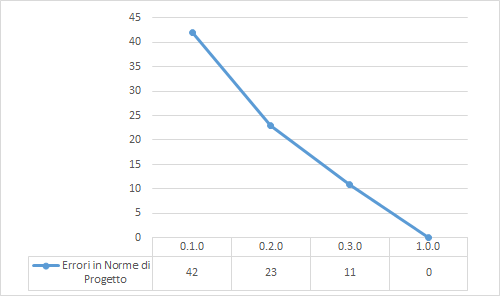
\includegraphics[width=10cm]{img/erroriNorme.png}
        \label{fig:scice_documenti}
        \caption{Grafico errori per \textsc{Norme Di Progetto v1.0.0-old}}
    \end{figure}

\paragraph{Studio di Fattibilità}
\label{sub:studio_di_fattibilita}
Essendo lo \textsc{Studio di Fattibilità v1.0.0-old} uno dei primi documenti redatti dal gruppo, il numero di errori è risultato alto rispetto al contenuto soprattutto per errori di dimenticanza nel rispettare quanto scritto nelle \textsc{Norme di Progetto v1.0.0-old}.
In questo documento sono state fatte 2 sole fasi di verifica in quanto il documento aveva contenuti più ristretti rispetto agli altri documenti e dopo la seconda verifica non vi sono stati aggiunti ulteriori contenuti.
Il risultato dell'indice di Gulpease è di 68 che soddisfa il valore accettabile dell'obiettivo.

\rowcolors{2}{white!80!lightgray!90}{white}
\renewcommand{\arraystretch}{2} % allarga le righe con dello spazio sotto e sopra
\begin{longtable}[H]{>{\centering\bfseries}m{6cm} >{\centering}m{2cm} >{\centering}m{2.5cm} >{\centering}m{2.5cm} >{\centering\arraybackslash}m{2.5cm}}  
  \rowcolor{lightgray}
  {\textbf{Documento}} & {\textbf{Risultato indice}} & {\textbf{Errori presenti}} & {\textbf{Esito indice}} & {\textbf{Esito errori}}  \\
  \endfirsthead%
  \rowcolor{lightgray}
  {\textbf{Documento}} & {\textbf{Risultato indice}} & {\textbf{Errori presenti}} & {\textbf{Esito indice}} & {\textbf{Esito errori}}  \\
  \endhead%
  \textbf{Studio di Fattibilità v1.0.0-old} & 68                 & 0               & Soddisfatto & Soddisfatto \\
  \caption{Risultati metriche per lo Studio di Fattibilità v1.0.0-old}
  \label{tab:my-table}
\end{longtable}

    \begin{figure}[H]
        \centering
        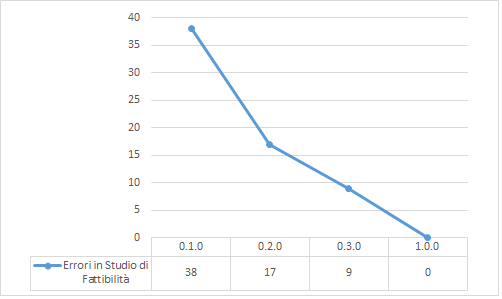
\includegraphics[width=10cm]{img/erroriStudio.png}
        \label{fig:scice_documenti}
        \caption{Grafico errori per \textsc{Studio di Fattibilità v1.0.0-old}}
    \end{figure}

\paragraph{Piano di Qualifica}
\label{sub:piano_di_qualifica}
Il \textsc{Piano di Qualifica vv1.0.0-old} ha presentato molti errori durante la sua realizzazione soprattutto nelle fasi di verifica in cui sono state realizzate le versioni 0.1.0 e 0.3.0 in quanto in quei periodi sono stati redatti gran parte dei contenuti del piano.
Essendo un documento ricco di sezioni e contenuti si è reso necessario effettuare 4 fasi di verifica per il documento.
L'indice di Gulpease, il cui risultato è 73, del documento rientra nel range definito tra 65 e 75.

\rowcolors{2}{white!80!lightgray!90}{white}
\renewcommand{\arraystretch}{2} % allarga le righe con dello spazio sotto e sopra
\begin{longtable}[H]{>{\centering\bfseries}m{6cm} >{\centering}m{2cm} >{\centering}m{2.5cm} >{\centering}m{2.5cm} >{\centering\arraybackslash}m{2.5cm}}  
  \rowcolor{lightgray}
  {\textbf{Documento}} & {\textbf{Risultato indice}} & {\textbf{Errori presenti}} & {\textbf{Esito indice}} & {\textbf{Esito errori}}  \\
  \endfirsthead%
  \rowcolor{lightgray}
  {\textbf{Documento}} & {\textbf{Risultato indice}} & {\textbf{Errori presenti}} & {\textbf{Esito indice}} & {\textbf{Esito errori}}  \\
  \endhead%
  \textbf{Piano di Qualifica v1.0.0-old} &  73               & 0               & Soddisfatto & Soddisfatto \\
  \caption{Risultati metriche per il Piano di Qualifica v1.0.0-old}
  \label{tab:my-table}
\end{longtable}

\begin{figure}[H]
    \centering
    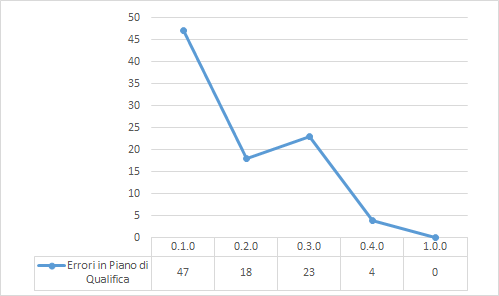
\includegraphics[width=10cm]{img/erroriPdQ.png}
    \label{fig:scice_documenti}
    \caption{Grafico errori per \textsc{Piano di Qualifica v1.0.0-old}}
\end{figure}

\paragraph{Piano di Progetto}
\label{sub:piano_di_progetto}
Il \textsc{Piano di Progetto v1.0.0-old} ha presentato parecchi errori inizialmente così come il \textsc{Piano di Qualifica v1.0.0-old} ma dopo ogni verifica il numero di errori è sceso in modo quasi lineare fino a raggiungere l'obiettivo di 0 errori prefissato.
L'indice di Gulpease rilevato, del documento è 75 che eguaglia il valore desiderabile dell'obiettivo.

\rowcolors{2}{white!80!lightgray!90}{white}
\renewcommand{\arraystretch}{2} % allarga le righe con dello spazio sotto e sopra
\begin{longtable}[H]{>{\centering\bfseries}m{6cm} >{\centering}m{2cm} >{\centering}m{2.5cm} >{\centering}m{2.5cm} >{\centering\arraybackslash}m{2.5cm}}  
  \rowcolor{lightgray}
  {\textbf{Documento}} & {\textbf{Risultato indice}} & {\textbf{Errori presenti}} & {\textbf{Esito indice}} & {\textbf{Esito errori}}  \\
  \endfirsthead%
  \rowcolor{lightgray}
  {\textbf{Documento}} & {\textbf{Risultato indice}} & {\textbf{Errori presenti}} & {\textbf{Esito indice}} & {\textbf{Esito errori}}  \\
  \endhead%
  \textbf{Piano di Progetto v1.0.0-old} & 75                 & 0               & Soddisfatto & Soddisfatto \\
  \caption{Risultati metriche per il Piano di Progetto v1.0.0-old}
  \label{tab:my-table}
\end{longtable}

\begin{figure}[H]
    \centering
    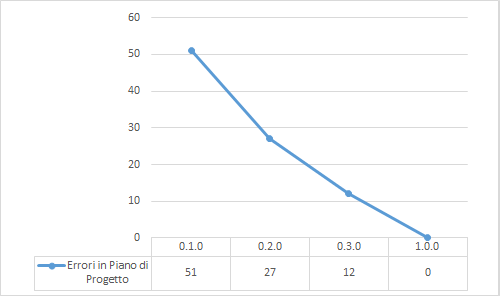
\includegraphics[width=10cm]{img/erroriPdP.png}
    \label{fig:scice_documenti}
    \caption{Grafico errori per \textsc{Piano di Progetto v1.0.0-old}}
\end{figure}

\paragraph{Analisi dei Requisiti}
\label{sub:analisi_dei_requisiti}
Come per le \textsc{Norme di Progetto v1.0.0-old} essendo anche l'\textsc{Analisi dei Requisiti v1.0.0-old} un documento abbastanza corposo il numero di errori rilevati durante le verifiche è stato elevato ma non eccessivo, inoltre si nota che nella fase di verifica che ha portato alla creazione della versione 0.3.0 il numero di errori è drasticamente calato. 
L'indice di Gulpease, essendo 73, rientra nel range desiderato per l'obiettivo.

\rowcolors{2}{white!80!lightgray!90}{white}
\renewcommand{\arraystretch}{2} % allarga le righe con dello spazio sotto e sopra
\begin{longtable}[H]{>{\centering\bfseries}m{6cm} >{\centering}m{2cm} >{\centering}m{2.5cm} >{\centering}m{2.5cm} >{\centering\arraybackslash}m{2.5cm}}  
  \rowcolor{lightgray}
  {\textbf{Documento}} & {\textbf{Risultato indice}} & {\textbf{Errori presenti}} & {\textbf{Esito indice}} & {\textbf{Esito errori}}  \\
  \endfirsthead%
  \rowcolor{lightgray}
  {\textbf{Documento}} & {\textbf{Risultato indice}} & {\textbf{Errori presenti}} & {\textbf{Esito indice}} & {\textbf{Esito errori}}  \\
  \endhead%
  \textbf{Analisi dei Requisiti v1.0.0-old} & 73                 & 0               & Soddisfatto & Soddisfatto \\
  \caption{Risultati metriche per l'Analisi dei Requisiti v1.0.0-old}
  \label{tab:my-table}
\end{longtable}

    \begin{figure}[H]
        \centering
        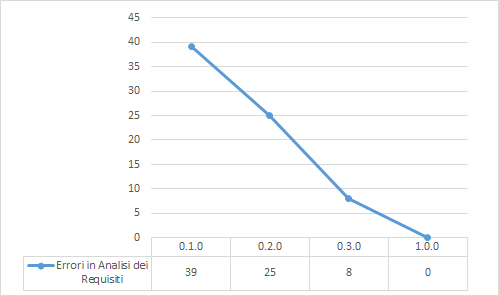
\includegraphics[width=10cm]{img/erroriAnalisi.png}
        \label{fig:scice_documenti}
        \caption{Grafico errori per \textsc{Analisi dei Requisiti v1.0.0-old}}
    \end{figure}

\paragraph{Glossario}
\label{sub:glossario}
Essendo il \textsc{Glossario v1.0.0-old} un documento abbastanza semplice e con lo scopo di informare il lettore sul significato di termini particolari, si è deciso di effettuare una sola fase di verifica finale.     
L'indice di Gulpease di questo documento è 65, che risulta essere al limite col valore accettabile, ma soddisfa comunque l'obiettivo.

\rowcolors{2}{white!80!lightgray!90}{white}
\renewcommand{\arraystretch}{2} % allarga le righe con dello spazio sotto e sopra
\begin{longtable}[H]{>{\centering\bfseries}m{6cm} >{\centering}m{2cm} >{\centering}m{2.5cm} >{\centering}m{2.5cm} >{\centering\arraybackslash}m{2.5cm}}  
  \rowcolor{lightgray}
  {\textbf{Documento}} & {\textbf{Risultato indice}} & {\textbf{Errori presenti}} & {\textbf{Esito indice}} & {\textbf{Esito errori}}  \\
  \endfirsthead%
  \rowcolor{lightgray}
  {\textbf{Documento}} & {\textbf{Risultato indice}} & {\textbf{Errori presenti}} & {\textbf{Esito indice}} & {\textbf{Esito errori}}  \\
  \endhead%
  \textbf{Glossario v1.0.0-old} & 65                 & 0               & Soddisfatto & Soddisfatto \\
  \caption{Risultati metriche per il Glossario v1.0.0-old}
  \label{tab:my-table}
\end{longtable}

\begin{figure}[H]
  \centering
  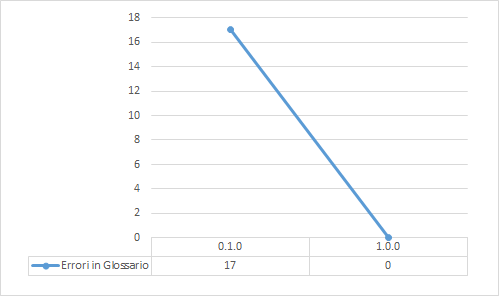
\includegraphics[width=10cm]{img/erroriGlossario.png}
  \label{fig:scice_documenti}
  \caption{Grafico errori per \textsc{Glossario v1.0.0-old}}
\end{figure}

\subsubsection{Esiti verifiche sui processi}
\label{sub:esiti_verifiche_sui_processi}
In questa sezione vengono visualizzati gli esiti delle metriche prese in considerazione per quanto riguarda i processi produttivi.
Come per i documenti, anche per queste metriche verrà fornito un esito che può essere soddisfacente o meno.

\paragraph{Processo PRC001}
\label{sub:processo_PRC001}

\rowcolors{2}{white!80!lightgray!90}{white}
\renewcommand{\arraystretch}{2} % allarga le righe con dello spazio sotto e sopra
\begin{longtable}[H]{>{\centering\bfseries}m{5cm} >{\centering}m{5cm} >{\centering}m{2.5cm} >{\centering\arraybackslash}m{2.5cm}}  
  \rowcolor{lightgray}
  {\textbf{Obiettivo}} & {\textbf{Metrica}} & {\textbf{Risultato}} & {\textbf{Esito}}  \\
  \endfirsthead%
  \rowcolor{lightgray}
  {\textbf{Obiettivo}} & {\textbf{Metrica}} & {\textbf{Risultato}} & {\textbf{Esito}}  \\
  \endhead%
  \textbf{QoPR001 Rispetto delle scadenze della pianificazione} & MoPR001 Varianza dei tempi & 1.31 & Soddisfatto \\
  \caption{Risultati metrica MoPR001}
  \label{tab:my-table}
\end{longtable}
\textbf{Nota}: Il ritardo medio, nel rispetto delle scadenze interne al gruppo, è stato di 1.31 giorni che soddisfa la metrica in quanto non sono stati superati i 2 giorni di media.

\rowcolors{2}{white!80!lightgray!90}{white}
\renewcommand{\arraystretch}{2} % allarga le righe con dello spazio sotto e sopra
\begin{longtable}[H]{>{\centering\bfseries}m{5cm} >{\centering}m{5cm} >{\centering}m{2.5cm} >{\centering\arraybackslash}m{2.5cm}}  
  \rowcolor{lightgray}
  {\textbf{Obiettivo}} & {\textbf{Metrica}} & {\textbf{Risultato}} & {\textbf{Esito}}  \\
  \endfirsthead%
  \rowcolor{lightgray}
  {\textbf{Obiettivo}} & {\textbf{Metrica}} & {\textbf{Risultato}} & {\textbf{Esito}}  \\
  \endhead%
  \textbf{QoPR002 Rispetto del budget istanziato} & MoPR002 Varianza dei costi & +40 & Soddisfatto \\
  \caption{Risultati metrica MoPR002}
  \label{tab:my-table}
\end{longtable}
\textbf{Nota}: La variazione rispetto al preventivo iniziale rientra nel range deciso per la metrica per cui l'obiettivo in questa fase è stato soddisfatto. L'aumento rilevato è: +40 euro;

\rowcolors{2}{white!80!lightgray!90}{white}
\renewcommand{\arraystretch}{2} % allarga le righe con dello spazio sotto e sopra
\begin{longtable}[H]{>{\centering\bfseries}m{5cm} >{\centering}m{5cm} >{\centering}m{2.5cm} >{\centering\arraybackslash}m{2.5cm}}  
  \rowcolor{lightgray}
  {\textbf{Obiettivo}} & {\textbf{Metrica}} & {\textbf{Risultato}} & {\textbf{Esito}}  \\
  \endfirsthead%
  \rowcolor{lightgray}
  {\textbf{Obiettivo}} & {\textbf{Metrica}} & {\textbf{Risultato}} & {\textbf{Esito}}  \\
  \endhead%
  \textbf{QoPR003 Rispetto del ciclo di vita scelto} & MoPR003 Aderenza agli standard & Livello di maturità: 2 Valutazione attributi: L & Non soddisfatto \\
  \caption{Risultati metrica MoPR003}
  \label{tab:my-table}
\end{longtable}
\textbf{Nota}: Essendo il progetto ancora nelle fasi iniziali è prevedibile che il livello di maturità desiderato non sia ancora stato soddisfatto in quanto il raggiungimento dell'obiettivo è fissato per la fine del progetto.

\rowcolors{2}{white!80!lightgray!90}{white}
\renewcommand{\arraystretch}{2} % allarga le righe con dello spazio sotto e sopra
\begin{longtable}[H]{>{\centering\bfseries}m{5cm} >{\centering}m{5cm} >{\centering}m{2.5cm} >{\centering\arraybackslash}m{2.5cm}}  
  \rowcolor{lightgray}
  {\textbf{Obiettivo}} & {\textbf{Metrica}} & {\textbf{Risultato}} & {\textbf{Esito}}  \\
  \endfirsthead%
  \rowcolor{lightgray}
  {\textbf{Obiettivo}} & {\textbf{Metrica}} & {\textbf{Risultato}} & {\textbf{Esito}}  \\
  \endhead%
  \textbf{QoPR004 Rispetto dei ruoli e identificazione nei prodotti} & MoPR004 Aderenza ai ruoli & 0 & Soddisfatto \\
  \caption{Risultati metrica MoPR004}
  \label{tab:my-table}
\end{longtable}
\textbf{Nota}: In ogni documento prodotto i ruoli sono stati identificati e rispettati.

\rowcolors{2}{white!80!lightgray!90}{white}
\renewcommand{\arraystretch}{2} % allarga le righe con dello spazio sotto e sopra
\begin{longtable}[H]{>{\centering\bfseries}m{5cm} >{\centering}m{5cm} >{\centering}m{2.5cm} >{\centering\arraybackslash}m{2.5cm}}  
  \rowcolor{lightgray}
  {\textbf{Obiettivo}} & {\textbf{Metrica}} & {\textbf{Risultato}} & {\textbf{Esito}}  \\
  \endfirsthead%
  \rowcolor{lightgray}
  {\textbf{Obiettivo}} & {\textbf{Metrica}} & {\textbf{Risultato}} & {\textbf{Esito}}  \\
  \endhead%
  \textbf{QoPR005 Rispetto del versionamento dei prodotti} & MoPR005 Controllo prodotti & 21.4 & Soddisfatto \\
  \caption{Risultati metrica MoPR005}
  \label{tab:my-table}
\end{longtable}
\textbf{Nota}: Essendo la media dei commit nella repository oltre il valore desiderabile (che era 20), l'obiettivo è pienamente soddisfatto.

\paragraph{Processo PRC003}
\label{sub:processo_PRC003}

\rowcolors{2}{white!80!lightgray!90}{white}
\renewcommand{\arraystretch}{2} % allarga le righe con dello spazio sotto e sopra
\begin{longtable}[H]{>{\centering\bfseries}m{5cm} >{\centering}m{5cm} >{\centering}m{2.5cm} >{\centering\arraybackslash}m{2.5cm}}  
  \rowcolor{lightgray}
  {\textbf{Obiettivo}} & {\textbf{Metrica}} & {\textbf{Risultato}} & {\textbf{Esito}}  \\
  \endfirsthead%
  \rowcolor{lightgray}
  {\textbf{Obiettivo}} & {\textbf{Metrica}} & {\textbf{Risultato}} & {\textbf{Esito}}  \\
  \endhead%
  \textbf{QoPR010 Rispetto nella redazione dei documenti} & MoPR011 Analisi documenti & 3 & Soddisfatto \\
  \caption{Risultati metrica MoPR011}
  \label{tab:my-table}
\end{longtable}
\textbf{Nota}: Tutti i documenti più corposi e discorsivi sono stati verificati almeno 3 volte, mentre per i documenti più esili di contenuti sono bastate 1 o 2 fasi di verifica. Nonostante tutto il team ritiene l'obiettivo comunque soddisfatto soprattutto per il fatto che non sono stati rilasciati documenti con errori.

\subsubsection{Conclusioni}%
\label{sub:conclusioni}
I dati analizzati esprimono un buon andamento del lavoro svolto dal team che si prefissa come obiettivo quello di continuare a migliorare sotto ogni aspetto relativo alle metriche e agli obiettivi prefissati.
Nei periodi prossimi di realizzazione del progetto il team cercherà di mantenere questi risultati e, se possibile, migliorarli specialmente negli obiettivi più carenti rilevati in questa fase iniziale.

\subsection{Secondo periodo (RP)}
\label{sub:secondo_periodo}
Nella seconda parte del progetto si è attuata una verifica più approfondita sui documenti, correggendo eventuali errori concettuali individuati nella prima fase di Revisione dei Requisiti.
Sono quindi state attuate verifiche e modifiche più specifiche ai documenti, e verifiche sul software, in particolare sul codice scritto per il \glossario{Proof of Concept}.
Come per il primo periodo, gli errori rilevati verranno trattati nella sezione appendice §C del documento.

\subsubsection{Esiti verifiche sui documenti}
\label{sub:esiti_verifiche_sui_documenti}
Sui documenti sono state utilizzate le metriche per:
    \begin{itemize}
        \item \textbf{Indice di Gulpease};
        \item \textbf{Correttezza lessicale/ortografica}.
    \end{itemize}
Per evitare risultati errati nel calcole dell'Indice di Gulpease si è deciso di non tenere in considerazione:
    \begin{itemize}
        \item Il frontespizio di ogni documento;
        \item Le tabelle presenti nei documenti;
        \item Il diario delle modifiche all'interno di ogni documento.
    \end{itemize}
Per quanto riguarda la correttezza lessicale/ortografica, gli errori trovati non verranno classificati ma semplicemente conteggiati uniformemente includendo anche errori derivati dal mancato rispetto delle convenzioni scritte nelle \textsc{Norme di Progetto v2.0.0}.
\\ Per ogni metrica di ogni documento verrà inoltre inserito l'esito dell'analisi che può avere risultato soddisfacente o non.

\paragraph{Norme di Progetto}
\label{sub:norme_di_progetto}
Le \textsc{Norme di Progetto v1.4-2.2.2} hanno subito parecchie modifiche e miglioramenti in base a diverse problematiche trattate anche nella sezione appendice B, il che ha portato ad un alternarsi di errori nelle diverse fasi di verifica e approvazione.
Il suo indice di Gulpease finale si è assestato intorno a 70.

\rowcolors{2}{white!80!lightgray!90}{white}
\renewcommand{\arraystretch}{2} % allarga le righe con dello spazio sotto e sopra
\begin{longtable}[H]{>{\centering\bfseries}m{6cm} >{\centering}m{2cm} >{\centering}m{2.5cm} >{\centering}m{2.5cm} >{\centering\arraybackslash}m{2.5cm}}  
  \rowcolor{lightgray}
  {\textbf{Documento}} & {\textbf{Risultato indice}} & {\textbf{Errori presenti}} & {\textbf{Esito indice}} & {\textbf{Esito errori}}  \\
  \endfirsthead%
  \rowcolor{lightgray}
  {\textbf{Documento}} & {\textbf{Risultato indice}} & {\textbf{Errori presenti}} & {\textbf{Esito indice}} & {\textbf{Esito errori}}  \\
  \endhead%
  \textbf{Norme di Progetto v1.4-2.2.2} & 70                 & 0               & Soddisfatto & Soddisfatto \\
  \caption{Risultati metriche per le Norme di Progetto v1.4-2.2.2}
  \label{tab:my-table}
\end{longtable}

\begin{figure}[H]
  \centering
  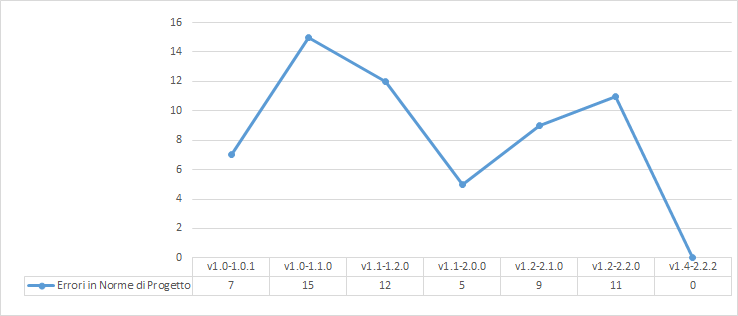
\includegraphics[width=10cm]{img/erroriNdPv1.4-2.2.2.png}
  \label{fig:errori_ndp}
  \caption{Grafico errori per \textsc{Norme di Progetto v1.4-2.2.2}}
\end{figure}

\begin{figure}[H]
  \centering
  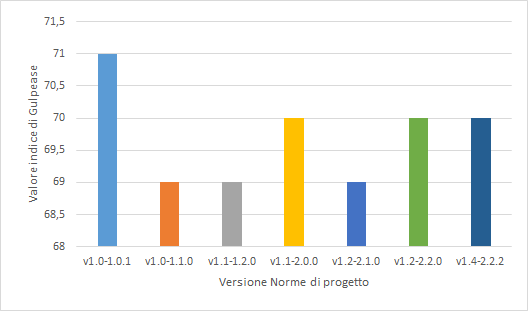
\includegraphics[width=10cm]{img/gulpeaseNdPv1.4-2.2.2.png}
  \label{fig:gulpease_ndp}
  \caption{Grafico indice di Gulpease per \textsc{Norme di Progetto v1.4-2.2.2}}
\end{figure}


\paragraph{Piano di Qualifica}
\label{sub:piano_di_qualifica}
Il \textsc{Piano di Qualifica v1.4-2.0.0} è stato verificato e approvato parecchie volte, nelle quali non sono stati individuati grandi quantità di errori nonostante le molte modifiche apportate ad esso.
Il suo indice di Gulpease è mutato leggermente nel tempo settandosi su un valore di 72 nell'ultima approvazione effettuata.

\rowcolors{2}{white!80!lightgray!90}{white}
\renewcommand{\arraystretch}{2} % allarga le righe con dello spazio sotto e sopra
\begin{longtable}[H]{>{\centering\bfseries}m{6cm} >{\centering}m{2cm} >{\centering}m{2.5cm} >{\centering}m{2.5cm} >{\centering\arraybackslash}m{2.5cm}}  
  \rowcolor{lightgray}
  {\textbf{Documento}} & {\textbf{Risultato indice}} & {\textbf{Errori presenti}} & {\textbf{Esito indice}} & {\textbf{Esito errori}}  \\
  \endfirsthead%
  \rowcolor{lightgray}
  {\textbf{Documento}} & {\textbf{Risultato indice}} & {\textbf{Errori presenti}} & {\textbf{Esito indice}} & {\textbf{Esito errori}}  \\
  \endhead%
  \textbf{Piano di Qualifica v1.4-2.0.0} & 72                & 0               & Soddisfatto & Soddisfatto \\
  \caption{Risultati metriche per il Piano di Qualifica v1.4-2.0.0}
  \label{tab:my-table}
\end{longtable}

\begin{figure}[H]
  \centering
  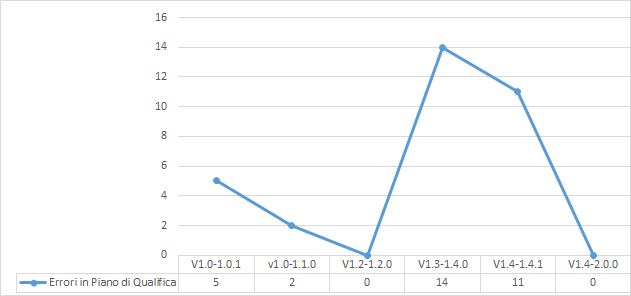
\includegraphics[width=10cm]{img/erroriPdQV1.4-2.0.0.png}
  \label{fig:errori_pdq}
  \caption{Grafico errori per \textsc{Piano di Qualifica v1.4-2.0.0}}
\end{figure}

\begin{figure}[H]
  \centering
  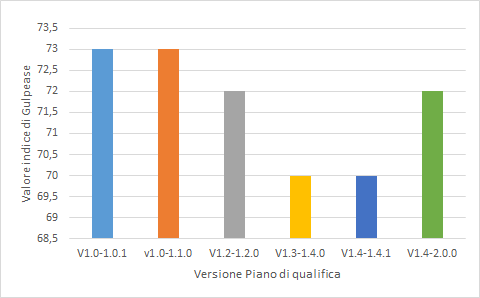
\includegraphics[width=10cm]{img/GulpeasePdQV1.4-2.0.0.png}
  \label{fig:gulpease_pdq}
  \caption{Grafico indice di Gulpease per \textsc{Piano di Qualifica v1.4-2.0.0}}
\end{figure}


\paragraph{Piano di Progetto}
\label{sub:piano_di_progetto}
Il \textsc{Piano di Progetto v1.4-3.1.0} ha subito molte modifiche durante questa fase di sviluppo, il che ha portato ad attuare molte fasi di verifica durante questo periodo di sviluppo del progetto.
Il suo indice di Gulpease è mutato leggermente nel tempo settandosi su un valore di 74 già nella v1.3-3.0.0.

\rowcolors{2}{white!80!lightgray!90}{white}
\renewcommand{\arraystretch}{2} % allarga le righe con dello spazio sotto e sopra
\begin{longtable}[H]{>{\centering\bfseries}m{6cm} >{\centering}m{2cm} >{\centering}m{2.5cm} >{\centering}m{2.5cm} >{\centering\arraybackslash}m{2.5cm}}  
  \rowcolor{lightgray}
  {\textbf{Documento}} & {\textbf{Risultato indice}} & {\textbf{Errori presenti}} & {\textbf{Esito indice}} & {\textbf{Esito errori}}  \\
  \endfirsthead%
  \rowcolor{lightgray}
  {\textbf{Documento}} & {\textbf{Risultato indice}} & {\textbf{Errori presenti}} & {\textbf{Esito indice}} & {\textbf{Esito errori}}  \\
  \endhead%
  \textbf{Piano di Progetto v1.4-3.1.0} & 74                 & 0               & Soddisfatto & Soddisfatto \\
  \caption{Risultati metriche per il Piano di Progetto v1.4-3.1.0}
  \label{tab:my-table}
\end{longtable}

\begin{figure}[H]
  \centering
  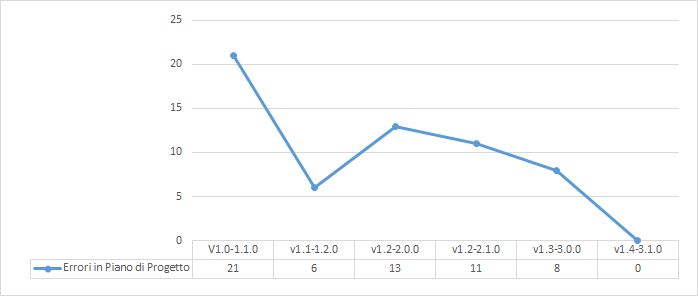
\includegraphics[width=10cm]{img/erroriPdPv1.4-3.1.0.png}
  \label{fig:errori_pdq}
  \caption{Grafico errori per \textsc{Piano di Progetto v1.4-3.1.0}}
\end{figure}

\begin{figure}[H]
  \centering
  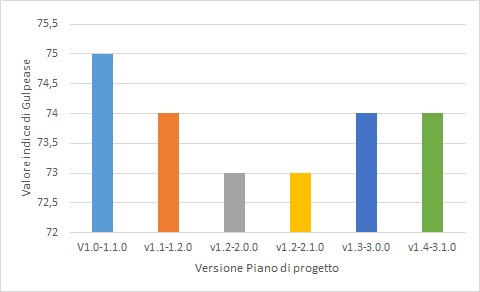
\includegraphics[width=10cm]{img/gulpeasePdPv1.4-3.1.0.png}
  \label{fig:gulpease_pdq}
  \caption{Grafico indice di Gulpease per \textsc{Piano di Progetto v1.4-3.1.0}}
\end{figure}


\paragraph{Analisi dei Requisiti}
\label{sub:analisi_dei_requisiti}
Nell' \textsc{Analisi dei Requisiti v1.4-1.2.1} le modifiche apportate fanno riferimento solamente ai casi d'uso al suo interno, il numero di errori rilevati è quindi contenuto e anche il numero di verifiche e approvazioni del documento è più basso rispetto agli altri documenti.
Il suo indice di Gulpease finale è rimasto a 73.

\rowcolors{2}{white!80!lightgray!90}{white}
\renewcommand{\arraystretch}{2} % allarga le righe con dello spazio sotto e sopra
\begin{longtable}[H]{>{\centering\bfseries}m{6cm} >{\centering}m{2cm} >{\centering}m{2.5cm} >{\centering}m{2.5cm} >{\centering\arraybackslash}m{2.5cm}}  
  \rowcolor{lightgray}
  {\textbf{Documento}} & {\textbf{Risultato indice}} & {\textbf{Errori presenti}} & {\textbf{Esito indice}} & {\textbf{Esito errori}}  \\
  \endfirsthead%
  \rowcolor{lightgray}
  {\textbf{Documento}} & {\textbf{Risultato indice}} & {\textbf{Errori presenti}} & {\textbf{Esito indice}} & {\textbf{Esito errori}}  \\
  \endhead%
  \textbf{Analisi dei Requisiti v1.4-1.2.1} & 73                 & 0               & Soddisfatto & Soddisfatto \\
  \caption{Risultati metriche per l'Analisi dei Requisiti v1.4-1.2.1}
  \label{tab:my-table}
\end{longtable}

\begin{figure}[H]
  \centering
  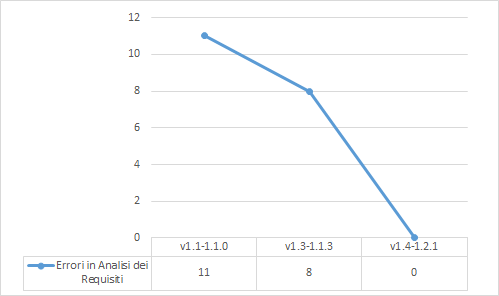
\includegraphics[width=10cm]{img/erroriAdRv1.4-1.2.1.png}
  \label{fig:errori_adr}
  \caption{Grafico errori per \textsc{Analisi dei Requisiti v1.4-1.2.1}}
\end{figure}

\begin{figure}[H]
  \centering
  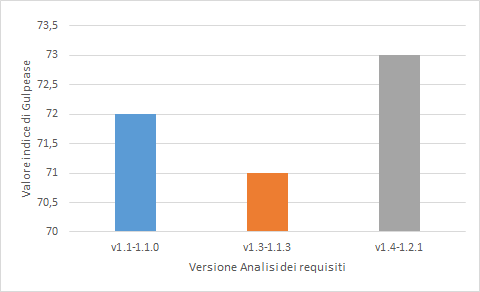
\includegraphics[width=10cm]{img/gulpeaseAdrv1.4-1.2.1.png}
  \label{fig:gulpease_adr}
  \caption{Grafico indice di Gulpease per \textsc{Analisi dei Requisiti v1.4-1.2.1}}
\end{figure}


\paragraph{Glossario}
\label{sub:glossario}
Il \textsc{Glossario v1.4-1.2.0} essendo un documento in cui sono state apportate poche modifiche significative, ha richiesto poche approvazioni e verifiche, dati i pochi errori riscontrati.
Il suo indice di Gulpease è rimasto immutato in ogni fase di approvazione rimanendo a 65.

\rowcolors{2}{white!80!lightgray!90}{white}
\renewcommand{\arraystretch}{2} % allarga le righe con dello spazio sotto e sopra
\begin{longtable}[H]{>{\centering\bfseries}m{6cm} >{\centering}m{2cm} >{\centering}m{2.5cm} >{\centering}m{2.5cm} >{\centering\arraybackslash}m{2.5cm}}  
  \rowcolor{lightgray}
  {\textbf{Documento}} & {\textbf{Risultato indice}} & {\textbf{Errori presenti}} & {\textbf{Esito indice}} & {\textbf{Esito errori}}  \\
  \endfirsthead%
  \rowcolor{lightgray}
  {\textbf{Documento}} & {\textbf{Risultato indice}} & {\textbf{Errori presenti}} & {\textbf{Esito indice}} & {\textbf{Esito errori}}  \\
  \endhead%
  \textbf{Glossario v1.4-1.2.0} & 65                 & 0               & Soddisfatto & Soddisfatto \\
  \caption{Risultati metriche per il Glossario v1.4-1.2.0}
  \label{tab:my-table}
\end{longtable}

\begin{figure}[H]
  \centering
  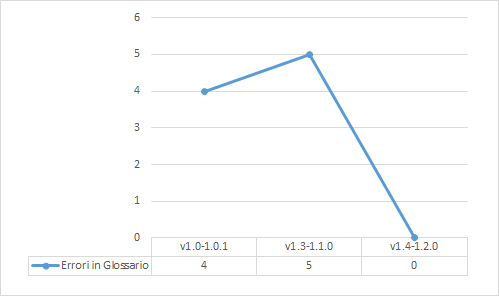
\includegraphics[width=10cm]{img/erroriGlosv1.4-1.2.0.png}
  \label{fig:errori_glos}
  \caption{Grafico errori per \textsc{Glossario v1.4-1.2.0}}
\end{figure}

\begin{figure}[H]
  \centering
  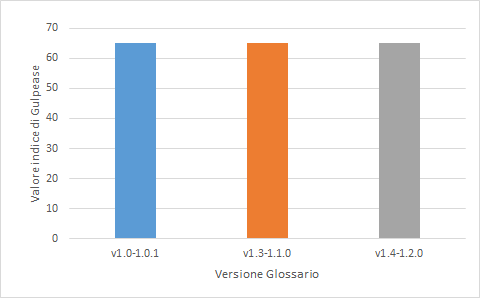
\includegraphics[width=10cm]{img/gulpeaseGlosv1.4-1.2.0.png}
  \label{fig:gulpease_glos}
  \caption{Grafico indice di Gulpease per \textsc{Glossario v1.4-1.2.0}}
\end{figure}

\subsubsection{Esiti verifiche sui processi}
\label{sub:esiti_verifiche_sui_processi}
In questa sezione vengono visualizzati gli esiti delle metriche prese in considerazione per quanto riguarda i processi produttivi.
Come per i documenti, anche per queste metriche verrà fornito un esito che può essere soddisfacente o meno.

\paragraph{Processo PRC001}
\label{sub:processo_PRC001}

\rowcolors{2}{white!80!lightgray!90}{white}
\renewcommand{\arraystretch}{2} % allarga le righe con dello spazio sotto e sopra
\begin{longtable}[H]{>{\centering\bfseries}m{5cm} >{\centering}m{5cm} >{\centering}m{2.5cm} >{\centering\arraybackslash}m{2.5cm}}  
  \rowcolor{lightgray}
  {\textbf{Obiettivo}} & {\textbf{Metrica}} & {\textbf{Risultato}} & {\textbf{Esito}}  \\
  \endfirsthead%
  \rowcolor{lightgray}
  {\textbf{Obiettivo}} & {\textbf{Metrica}} & {\textbf{Risultato}} & {\textbf{Esito}}  \\
  \endhead%
  \textbf{QoPR001 Rispetto delle scadenze della pianificazione} & MoPR001 Varianza dei tempi & 1.10  & Soddisfatto  \\
  \caption{Risultati metrica MoPR001}
  \label{tab:my-table}
\end{longtable}
\textbf{Nota}: Il valore della varianza dei tempi è migliorato rispetto alla prima fase e rientra ancora nel valore accettabile definito dal gruppo.

\rowcolors{2}{white!80!lightgray!90}{white}
\renewcommand{\arraystretch}{2} % allarga le righe con dello spazio sotto e sopra
\begin{longtable}[H]{>{\centering\bfseries}m{5cm} >{\centering}m{5cm} >{\centering}m{2.5cm} >{\centering\arraybackslash}m{2.5cm}}  
  \rowcolor{lightgray}
  {\textbf{Obiettivo}} & {\textbf{Metrica}} & {\textbf{Risultato}} & {\textbf{Esito}}  \\
  \endfirsthead%
  \rowcolor{lightgray}
  {\textbf{Obiettivo}} & {\textbf{Metrica}} & {\textbf{Risultato}} & {\textbf{Esito}}  \\
  \endhead%
  \textbf{QoPR002 Rispetto del budget istanziato} & MoPR002 Varianza dei costi & -2 & Soddisfatto  \\
  \caption{Risultati metrica MoPR002}
  \label{tab:my-table}
\end{longtable}
\textbf{Nota}: La variazione rispetto al preventivo iniziale rientra nel range deciso per la metrica, per cui l’obiettivo è stato soddisfatto. Il discostamento dal preventivo totale rilevato è di: -2 euro;

\rowcolors{2}{white!80!lightgray!90}{white}
\renewcommand{\arraystretch}{2} % allarga le righe con dello spazio sotto e sopra
\begin{longtable}[H]{>{\centering\bfseries}m{5cm} >{\centering}m{5cm} >{\centering}m{2.5cm} >{\centering\arraybackslash}m{2.5cm}}  
  \rowcolor{lightgray}
  {\textbf{Obiettivo}} & {\textbf{Metrica}} & {\textbf{Risultato}} & {\textbf{Esito}}  \\
  \endfirsthead%
  \rowcolor{lightgray}
  {\textbf{Obiettivo}} & {\textbf{Metrica}} & {\textbf{Risultato}} & {\textbf{Esito}}  \\
  \endhead%
  \textbf{QoPR003 Rispetto del ciclo di vita scelto} & MoPR003 Aderenza agli standard & Livello di maturità:  2 \\ Valutazione attributi:  L &  Non soddisfatto \\
  \caption{Risultati metrica MoPR003}
  \label{tab:my-table}
\end{longtable}
\textbf{Nota}: Si è intravisto un miglioramento all'interno del gruppo per quanto riguarda l'aderenza agli standard, ma non ancora sufficiente per gli obiettivi prefissati.

\rowcolors{2}{white!80!lightgray!90}{white}
\renewcommand{\arraystretch}{2} % allarga le righe con dello spazio sotto e sopra
\begin{longtable}[H]{>{\centering\bfseries}m{5cm} >{\centering}m{5cm} >{\centering}m{2.5cm} >{\centering\arraybackslash}m{2.5cm}}  
  \rowcolor{lightgray}
  {\textbf{Obiettivo}} & {\textbf{Metrica}} & {\textbf{Risultato}} & {\textbf{Esito}}  \\
  \endfirsthead%
  \rowcolor{lightgray}
  {\textbf{Obiettivo}} & {\textbf{Metrica}} & {\textbf{Risultato}} & {\textbf{Esito}}  \\
  \endhead%
  \textbf{QoPR004 Rispetto dei ruoli e identificazione nei prodotti} & MoPR004 Aderenza ai ruoli & 0 & Soddisfatto \\
  \caption{Risultati metrica MoPR004}
  \label{tab:my-table}
\end{longtable}
\textbf{Nota}: In ogni documento prodotto i ruoli sono stati identificati e rispettati.

\rowcolors{2}{white!80!lightgray!90}{white}
\renewcommand{\arraystretch}{2} % allarga le righe con dello spazio sotto e sopra
\begin{longtable}[H]{>{\centering\bfseries}m{5cm} >{\centering}m{5cm} >{\centering}m{2.5cm} >{\centering\arraybackslash}m{2.5cm}}  
  \rowcolor{lightgray}
  {\textbf{Obiettivo}} & {\textbf{Metrica}} & {\textbf{Risultato}} & {\textbf{Esito}}  \\
  \endfirsthead%
  \rowcolor{lightgray}
  {\textbf{Obiettivo}} & {\textbf{Metrica}} & {\textbf{Risultato}} & {\textbf{Esito}}  \\
  \endhead%
  \textbf{QoPR005 Rispetto del versionamento dei prodotti} & MoPR005 Controllo prodotti & 29.8 & Soddisfatto \\
  \caption{Risultati metrica MoPR005}
  \label{tab:my-table}
\end{longtable}
\textbf{Nota}: Il numero di commit in questa fase è stato parecchio elevato, il che soddisfa appieno l'obiettivo prefissato per questa norma.

\paragraph{Processo PRC002}
\label{sub:processo_PRC002}

\rowcolors{2}{white!80!lightgray!90}{white}
\renewcommand{\arraystretch}{2} % allarga le righe con dello spazio sotto e sopra
\begin{longtable}[H]{>{\centering\bfseries}m{5cm} >{\centering}m{5cm} >{\centering}m{2.5cm} >{\centering\arraybackslash}m{2.5cm}}  
  \rowcolor{lightgray}
  {\textbf{Obiettivo}} & {\textbf{Metrica}} & {\textbf{Risultato}} & {\textbf{Esito}}  \\
  \endfirsthead%
  \rowcolor{lightgray}
  {\textbf{Obiettivo}} & {\textbf{Metrica}} & {\textbf{Risultato}} & {\textbf{Esito}}  \\
  \endhead%
  \textbf{QoPR006 Soddisfazione dei requisiti obbligatori} & MoPR006 Verifica requisiti obbligatori & / & Non soddisfatto \\
  \caption{Risultati metrica MoPR006}
  \label{tab:my-table}
\end{longtable}
\textbf{Nota}: La revisione dei requisiti obbligatori soddisfatti non è ancora stata eseguita.

\rowcolors{2}{white!80!lightgray!90}{white}
\renewcommand{\arraystretch}{2} % allarga le righe con dello spazio sotto e sopra
\begin{longtable}[H]{>{\centering\bfseries}m{5cm} >{\centering}m{5cm} >{\centering}m{2.5cm} >{\centering\arraybackslash}m{2.5cm}}  
  \rowcolor{lightgray}
  {\textbf{Obiettivo}} & {\textbf{Metrica}} & {\textbf{Risultato}} & {\textbf{Esito}}  \\
  \endfirsthead%
  \rowcolor{lightgray}
  {\textbf{Obiettivo}} & {\textbf{Metrica}} & {\textbf{Risultato}} & {\textbf{Esito}}  \\
  \endhead%
  \textbf{QoPR007 Soddisfazione dei requisiti opzionali e desiderabili} & MoPR007 Verifica requisiti opzionali \\ MoPR008 Verifica requisiti desiderabili & / & Non soddisfatto \\
  \caption{Risultati metrica MoPR007 e metrica MoPR008}
  \label{tab:my-table}
\end{longtable}
\textbf{Nota}: La revisione dei requisiti opzionali e desiderabili soddisfatti non è ancora stata eseguita.

\rowcolors{2}{white!80!lightgray!90}{white}
\renewcommand{\arraystretch}{2} % allarga le righe con dello spazio sotto e sopra
\begin{longtable}[H]{>{\centering\bfseries}m{5cm} >{\centering}m{5cm} >{\centering}m{2.5cm} >{\centering\arraybackslash}m{2.5cm}}  
  \rowcolor{lightgray}
  {\textbf{Obiettivo}} & {\textbf{Metrica}} & {\textbf{Risultato}} & {\textbf{Esito}}  \\
  \endfirsthead%
  \rowcolor{lightgray}
  {\textbf{Obiettivo}} & {\textbf{Metrica}} & {\textbf{Risultato}} & {\textbf{Esito}}  \\
  \endhead%
  \textbf{QoPR008 Verifica dei rischi previsti} & MoPR009 Verifica rischi non pervenuti & 0 & Soddisfatto \\
  \caption{Risultati metrica MoPR009}
  \label{tab:my-table}
\end{longtable}
\textbf{Nota}: Non sono ancora stati rivelati rischi importanti che non siano stati previsti precedentemente dal gruppo.

\paragraph{Processo PRC003}
\label{sub:processo_PRC003}

\rowcolors{2}{white!80!lightgray!90}{white}
\renewcommand{\arraystretch}{2} % allarga le righe con dello spazio sotto e sopra
\begin{longtable}[H]{>{\centering\bfseries}m{5cm} >{\centering}m{5cm} >{\centering}m{2.5cm} >{\centering\arraybackslash}m{2.5cm}}  
  \rowcolor{lightgray}
  {\textbf{Obiettivo}} & {\textbf{Metrica}} & {\textbf{Risultato}} & {\textbf{Esito}}  \\
  \endfirsthead%
  \rowcolor{lightgray}
  {\textbf{Obiettivo}} & {\textbf{Metrica}} & {\textbf{Risultato}} & {\textbf{Esito}}  \\
  \endhead%
  \textbf{QoPR09 Rispetto delle fasi del ciclo di vita} & MoPR010 Analisi Way of Working & / & Soddisfatto \\
  \caption{Risultati metrica MoPR010}
  \label{tab:my-table}
\end{longtable}
\textbf{Nota}: I componenti del gruppo svolgono costantemente un aggiornamento in base alle modifiche fatte alle \textsc{Norme di Progetto v1.4-2.2.2}.

\rowcolors{2}{white!80!lightgray!90}{white}
\renewcommand{\arraystretch}{2} % allarga le righe con dello spazio sotto e sopra
\begin{longtable}[H]{>{\centering\bfseries}m{5cm} >{\centering}m{5cm} >{\centering}m{2.5cm} >{\centering\arraybackslash}m{2.5cm}}  
  \rowcolor{lightgray}
  {\textbf{Obiettivo}} & {\textbf{Metrica}} & {\textbf{Risultato}} & {\textbf{Esito}}  \\
  \endfirsthead%
  \rowcolor{lightgray}
  {\textbf{Obiettivo}} & {\textbf{Metrica}} & {\textbf{Risultato}} & {\textbf{Esito}}  \\
  \endhead%
  \textbf{QoPR010 Rispetto nella redazione dei documenti} & MoPR011 Analisi documenti & 4+ & Soddisfatto \\
  \caption{Risultati metrica MoPR011}
  \label{tab:my-table}
\end{longtable}
\textbf{Nota}: Tutti i documenti più corposi sono stati verificati almeno 4 volte, il che soddisfa pienamente le aspettative del gruppo.

\paragraph{Processo PRC004}
\label{sub:processo_PRC004}

\rowcolors{2}{white!80!lightgray!90}{white}
\renewcommand{\arraystretch}{2} % allarga le righe con dello spazio sotto e sopra
\begin{longtable}[H]{>{\centering\bfseries}m{5cm} >{\centering}m{5cm} >{\centering}m{2.5cm} >{\centering\arraybackslash}m{2.5cm}}  
  \rowcolor{lightgray}
  {\textbf{Obiettivo}} & {\textbf{Metrica}} & {\textbf{Risultato}} & {\textbf{Esito}}  \\
  \endfirsthead%
  \rowcolor{lightgray}
  {\textbf{Obiettivo}} & {\textbf{Metrica}} & {\textbf{Risultato}} & {\textbf{Esito}}  \\
  \endhead%
  \textbf{QoPR011 Attuare una verifica costante} & MoPR012 Frequenza di controlli & / & Soddisfatto \\
  \caption{Risultati metrica MoPR012}
  \label{tab:my-table}
\end{longtable}
\textbf{Nota}: I verificatori stanno continuando ad effettuare delle verifiche costanti ai prodotti.


\rowcolors{2}{white!80!lightgray!90}{white}
\renewcommand{\arraystretch}{2} % allarga le righe con dello spazio sotto e sopra
\begin{longtable}[H]{>{\centering\bfseries}m{5cm} >{\centering}m{5cm} >{\centering}m{2.5cm} >{\centering\arraybackslash}m{2.5cm}}  
  \rowcolor{lightgray}
  {\textbf{Obiettivo}} & {\textbf{Metrica}} & {\textbf{Risultato}} & {\textbf{Esito}}  \\
  \endfirsthead%
  \rowcolor{lightgray}
  {\textbf{Obiettivo}} & {\textbf{Metrica}} & {\textbf{Risultato}} & {\textbf{Esito}}  \\
  \endhead%
  \textbf{QoPR013 Rispettare le fasi di verifica} & MoPR010 Analisi Way of Working & / & Soddisfatto \\
  \caption{Risultati QoPR13}
  \label{tab:my-table}
\end{longtable}
\textbf{Nota}: Le fasi di verifica dei prodotti stanno vedendo rispettate secondo le indicazioni interne al gruppo.

\rowcolors{2}{white!80!lightgray!90}{white}
\renewcommand{\arraystretch}{2} % allarga le righe con dello spazio sotto e sopra
\begin{longtable}[H]{>{\centering\bfseries}m{5cm} >{\centering}m{5cm} >{\centering}m{2.5cm} >{\centering\arraybackslash}m{2.5cm}}  
  \rowcolor{lightgray}
  {\textbf{Obiettivo}} & {\textbf{Metrica}} & {\textbf{Risultato}} & {\textbf{Esito}}  \\
  \endfirsthead%
  \rowcolor{lightgray}
  {\textbf{Obiettivo}} & {\textbf{Metrica}} & {\textbf{Risultato}} & {\textbf{Esito}}  \\
  \endhead%
  \textbf{QoPR014 Soddisfare i test richiesti} & MoPR013 Percentuale di test soddisfatti & 0\% & Non soddisfatto \\
  \caption{Risultati MoPR013}
  \label{tab:my-table}
\end{longtable}
\textbf{Nota}: L'obiettivo per questa metrica non è ancora stato soddisfatto in quanto l'implementazione dei test avverrà nel prossimo periodo di sviluppo.

\subsubsection{Esiti verifiche sui prodotti}
\label{sub:esiti_verifiche_sui_prodotti}
In questa sezione vengono visualizzati gli esiti delle metriche prese in considerazione per quanto riguarda i prodotti realizzati. Come per i documenti, anche per queste metriche verrà fornito un esito che può essere soddisfacente o meno.

\paragraph{Funzionalità}
\label{sub:funzionalita}

\rowcolors{2}{white!80!lightgray!90}{white}
\renewcommand{\arraystretch}{2} % allarga le righe con dello spazio sotto e sopra
\begin{longtable}[H]{>{\centering\bfseries}m{5cm} >{\centering}m{5cm} >{\centering}m{2.5cm} >{\centering\arraybackslash}m{2.5cm}}  
  \rowcolor{lightgray}
  {\textbf{Obiettivo}} & {\textbf{Metrica}} & {\textbf{Risultato}} & {\textbf{Esito}}  \\
  \endfirsthead%
  \rowcolor{lightgray}
  {\textbf{Obiettivo}} & {\textbf{Metrica}} & {\textbf{Risultato}} & {\textbf{Esito}}  \\
  \endhead%
  \textbf{QoPD001 Rispetto dell’implementazione funzionale - [Adeguatezza]} & MoPD001 Completezza di implementazione - [Adeguatezza] & / & Non Soddisfatto \\
  \caption{Risultati metrica MoPD001}
  \label{tab:my-table}
\end{longtable}
\textbf{Nota}: Questa metrica risulta essere 0 in quanto in questa fase di sviluppo non sono ancora state definite chiaramente le funzioni totali da realizzare.

\rowcolors{2}{white!80!lightgray!90}{white}
\renewcommand{\arraystretch}{2} % allarga le righe con dello spazio sotto e sopra
\begin{longtable}[H]{>{\centering\bfseries}m{5cm} >{\centering}m{5cm} >{\centering}m{2.5cm} >{\centering\arraybackslash}m{2.5cm}}  
  \rowcolor{lightgray}
  {\textbf{Obiettivo}} & {\textbf{Metrica}} & {\textbf{Risultato}} & {\textbf{Esito}}  \\
  \endfirsthead%
  \rowcolor{lightgray}
  {\textbf{Obiettivo}} & {\textbf{Metrica}} & {\textbf{Risultato}} & {\textbf{Esito}}  \\
  \endhead%
  \textbf{QoPD002 Rispetto delle interfacce - [Interoperabilità]} & MoPD002 Coerenza di interfaccia - [Interoperabilità] & / & Non soddisfatto \\
  \caption{Risultati metrica MoPD002}
  \label{tab:my-table}
\end{longtable}
\textbf{Nota}: Il totale delle interfacce delle funzioni non è ancora stato definito.

\paragraph{Affidabilità}
\label{sub:affidabilita}

\rowcolors{2}{white!80!lightgray!90}{white}
\renewcommand{\arraystretch}{2} % allarga le righe con dello spazio sotto e sopra
\begin{longtable}[H]{>{\centering\bfseries}m{5cm} >{\centering}m{5cm} >{\centering}m{2.5cm} >{\centering\arraybackslash}m{2.5cm}}  
  \rowcolor{lightgray}
  {\textbf{Obiettivo}} & {\textbf{Metrica}} & {\textbf{Risultato}} & {\textbf{Esito}}  \\
  \endfirsthead%
  \rowcolor{lightgray}
  {\textbf{Obiettivo}} & {\textbf{Metrica}} & {\textbf{Risultato}} & {\textbf{Esito}}  \\
  \endhead%
  \textbf{QoPD003 Test completi sul codice - [Maturità]} & MoPD003 Copertura dei test- [Maturità] & / & Non soddisfatto \\
  \caption{Risultati metrica MoPD003}
  \label{tab:my-table}
\end{longtable}
\textbf{Nota}: Per il Proof of concept non è stato implementato un sistema di copertura dei test automatico.

\rowcolors{2}{white!80!lightgray!90}{white}
\renewcommand{\arraystretch}{2} % allarga le righe con dello spazio sotto e sopra
\begin{longtable}[H]{>{\centering\bfseries}m{5cm} >{\centering}m{5cm} >{\centering}m{2.5cm} >{\centering\arraybackslash}m{2.5cm}}  
  \rowcolor{lightgray}
  {\textbf{Obiettivo}} & {\textbf{Metrica}} & {\textbf{Risultato}} & {\textbf{Esito}}  \\
  \endfirsthead%
  \rowcolor{lightgray}
  {\textbf{Obiettivo}} & {\textbf{Metrica}} & {\textbf{Risultato}} & {\textbf{Esito}}  \\
  \endhead%
  \textbf{QoPD004 Individuazione test falliti - [Affidabilità]} & MoPD004 Densità degli errori - [Affidabilità] & / & Non Soddisfatto \\
  \caption{Risultati metrica MoPD004}
  \label{tab:my-table}
\end{longtable}
\textbf{Nota}: Visto il non implemento di un sistema di copertura dei test automatico per il Proof of concept, non è stato possibile verificare il numero di test falliti.

\paragraph{Usabilità}
\label{sub:usabilita}

\rowcolors{2}{white!80!lightgray!90}{white}
\renewcommand{\arraystretch}{2} % allarga le righe con dello spazio sotto e sopra
\begin{longtable}[H]{>{\centering\bfseries}m{5cm} >{\centering}m{5cm} >{\centering}m{2.5cm} >{\centering\arraybackslash}m{2.5cm}}  
  \rowcolor{lightgray}
  {\textbf{Obiettivo}} & {\textbf{Metrica}} & {\textbf{Risultato}} & {\textbf{Esito}}  \\
  \endfirsthead%
  \rowcolor{lightgray}
  {\textbf{Obiettivo}} & {\textbf{Metrica}} & {\textbf{Risultato}} & {\textbf{Esito}}  \\
  \endhead%
  \textbf{QoPD005 Chiarezza del comportamento - [Comprensibilità]} & MoPD005 Documentazione delle funzioni - [Comprensibilità] & 30\%  & Non soddisfatto \\
  \caption{Risultati metrica MoPD005}
  \label{tab:my-table}
\end{longtable}
\textbf{Nota}: La percentuale di funzioni documentate con un commento è inferiore rispetto a quanto prefissate, il gruppo si impegnerà però a risolvere questa mancanza nella prossima fase di sviluppo.

\rowcolors{2}{white!80!lightgray!90}{white}
\renewcommand{\arraystretch}{2} % allarga le righe con dello spazio sotto e sopra
\begin{longtable}[H]{>{\centering\bfseries}m{5cm} >{\centering}m{5cm} >{\centering}m{2.5cm} >{\centering\arraybackslash}m{2.5cm}}  
  \rowcolor{lightgray}
  {\textbf{Obiettivo}} & {\textbf{Metrica}} & {\textbf{Risultato}} & {\textbf{Esito}}  \\
  \endfirsthead%
  \rowcolor{lightgray}
  {\textbf{Obiettivo}} & {\textbf{Metrica}} & {\textbf{Risultato}} & {\textbf{Esito}}  \\
  \endhead%
  \textbf{QoPD006 Chiarimento degli errori - [Comprensibilità]} & MoPD006 Messaggi di errore - [Comprensibilità] & 10\% & Soddisfatto \\
  \caption{Risultati metrica MoPD006}
  \label{tab:my-table}
\end{longtable}
\textbf{Nota}: Il valore della metrica è alto ma soddisfacente, anche perché il numero di messaggi di errore da gestire è ancora ristretto.

\paragraph{Efficienza}
\label{sub:efficienza}

\rowcolors{2}{white!80!lightgray!90}{white}
\renewcommand{\arraystretch}{2} % allarga le righe con dello spazio sotto e sopra
\begin{longtable}[H]{>{\centering\bfseries}m{5cm} >{\centering}m{5cm} >{\centering}m{2.5cm} >{\centering\arraybackslash}m{2.5cm}}  
  \rowcolor{lightgray}
  {\textbf{Obiettivo}} & {\textbf{Metrica}} & {\textbf{Risultato}} & {\textbf{Esito}}  \\
  \endfirsthead%
  \rowcolor{lightgray}
  {\textbf{Obiettivo}} & {\textbf{Metrica}} & {\textbf{Risultato}} & {\textbf{Esito}}  \\
  \endhead%
  \textbf{QoPD007 Velocità di esecuzione - [Comportamento temporale]} & MoPD007 Tempo medio di risposta - [Comportamento temporale] & minore di 1 sec. & Soddisfatto \\
  \caption{Risultati metrica MoPD007}
  \label{tab:my-table}
\end{longtable}
\textbf{Nota}: Il tempo di risposta soddisfa le aspettative di qualità anche se le funzionalità totali del programma realizzato per il Proof of concept rimangono ancora in numero ristretto.

\paragraph{Manutenibilità}
\label{sub:manutenibilita}

\rowcolors{2}{white!80!lightgray!90}{white}
\renewcommand{\arraystretch}{2} % allarga le righe con dello spazio sotto e sopra
\begin{longtable}[H]{>{\centering\bfseries}m{5cm} >{\centering}m{5cm} >{\centering}m{2.5cm} >{\centering\arraybackslash}m{2.5cm}}  
  \rowcolor{lightgray}
  {\textbf{Obiettivo}} & {\textbf{Metrica}} & {\textbf{Risultato}} & {\textbf{Esito}}  \\
  \endfirsthead%
  \rowcolor{lightgray}
  {\textbf{Obiettivo}} & {\textbf{Metrica}} & {\textbf{Risultato}} & {\textbf{Esito}}  \\
  \endhead%
  \textbf{QoPD08 Comprensione del codice - [Modifica]} & MoPD008 Commenti sul codice - [Modifica] & 5.36\% & Non soddisfatto \\
  \caption{Risultati metrica MoPD006}
  \label{tab:my-table}
\end{longtable}
\textbf{Nota}: Il risultato della metrica non soddisfa le aspettative del gruppo che si prefissa come obiettivo principale quello di aumentare il numero di commenti significativi all'interno del codice.

\subsubsection{Conclusioni}%
\label{sub:conclusioni}
Il gruppo si ritiene soddisfatto dell'andamento dello sviluppo soprattutto analizzando i dati degli esiti delle metriche più significative sui processi, nota però una grande opportunità di miglioramento specialmente nelle metriche riguardanti i prodotti, soprattutto di natura software.
Da quest'ultima riflessione il gruppo si impegna a mantenere un buon andamento dello sviluppo, cercando di migliorare significativamente le metriche riguardanti gli obiettivi dei prodotti.
\end{document}
